\chapter{Lanzadores}
\minitoc

La selección del vehículo de lanzamiento para misiones de pequeños satélites requiere priorizar la viabilidad económica mediante servicios de \textit{rideshare}. Esta modalidad permite distribuir los costes de lanzamiento entre múltiples operadores, reduciendo significativamente los gastos para cargas útiles pequeñas \cite{spacex2022}.

Los lanzamientos \textit{rideshare} han revolucionado el acceso al espacio para satélites de masa reducida. Utilizan adaptadores especializados y \textit{dispensers} para integrar múltiples cargas útiles en la etapa superior del cohete \cite{esa2024}. Esta estrategia ha democratizado las misiones espaciales, especialmente para proyectos académicos y empresas emergentes, reduciendo costes hasta un 90\% comparado con lanzamientos dedicados \cite{lionnet2025}.

\section{Lanzadores Operativos}

\subsection{Falcon 9}

Falcon 9 de SpaceX domina el mercado de \textit{rideshare} con su programa SmallSat Rideshare. Con 468 lanzamientos hasta abril de 2025 y una fiabilidad del 99.35\%, su desempeño supera ampliamente a competidores \cite{satellitetoday2024}. El programa Transporter ofrece lanzamientos dedicados a órbitas heliosíncronas con un coste de 6,500 USD por kilogramo \cite{spacex2022, payloadspace2023}. Su arquitectura de 9 motores Merlin proporciona redundancia crítica, mientras que su segunda etapa criogénica permite ajustes orbitales precisos para inserción en órbitas de hasta 700 km \cite{wikipedia2024}.

\subsection{Firefly Alpha}

El Firefly Alpha es un lanzador de dos etapas desarrollado por Firefly Aerospace para el mercado de satélites pequeños . Con una capacidad de 630 kg a órbitas heliosíncronas de 500 km y 1,030 kg a LEO, ocupa un nicho intermedio en el mercado . Hasta junio de 2025, ha completado 6 lanzamientos con una fiabilidad del 33.3\% (considerando solo éxitos completos). El coste de lanzamiento oscila entre 15-19 millones USD, resultando en aproximadamente 24,000-30,000 USD por kilogramo . Opera desde Vandenberg Space Force Base y ofrece opciones de rideshare limitadas \cite{fireflyspace2024}.

\subsection{Vulcan Centaur}

El Vulcan Centaur es el sucesor estadounidense del Atlas V y Delta IV Heavy. Aunque proyecta una fiabilidad del 100\% basada en pruebas iniciales, carece de historial operativo extenso en 2025 \cite{semanticscholar2023}. Su capacidad de 14,400 kg a SSO y coste aproximado de 110 millones USD lo posicionan fuera del segmento económico para satélites pequeños. La ausencia de servicios \textit{rideshare} establecidos limita su competitividad.

\subsection{Electron}

El Electron se especializa en cargas útiles ligeras con lanzamientos rápidos desde Nueva Zelanda. Su coste de 7.5 millones USD por lanzamiento resulta en aproximadamente 25,000 USD por kilogramo \cite{spaceinsider2023}. Con capacidad máxima de 300 kg a SSO, ofrece servicios \textit{rideshare} limitados pero flexibilidad operativa elevada con varias ventanas de lanzamiento \cite{wikipedia2024}.

\subsection{Ariane 6}

El Ariane 6 representa la autonomía estratégica europea en acceso al espacio. Sus variantes Ariane 62 y Ariane 64 ofrecen capacidades de 6,500 kg y 15,000 kg a SSO respectivamente \cite{esa2024}. Los servicios \textit{rideshare} permiten costes aproximados de 11.164,55 USD por kilogramo \cite{arstechnica2023}. Su etapa superior con capacidad de reinicio múltiple optimiza la inserción orbital para múltiples cargas útiles \cite{esa2024}.

\subsection{Vega-C}

El Vega-C es el lanzador ligero más avanzado de Europa, optimizado para el segmento de satélites pequeños y medianos. Con capacidad de 2,300 kg a órbitas de 700 km, utiliza el adaptador SSMS (Small Spacecraft Mission Service) para facilitar misiones \textit{rideshare} \cite{arianespace2024}. Los costes aproximados de 20,000 USD por kilogramo reflejan su especialización en el mercado europeo \cite{esa2024}.
\\
\begin{table}[h]
\centering
\caption{Comparativa de lanzadores espaciales para misiones \textit{rideshare}.}
\begin{tabularx}{\linewidth}{l X X X X X}
\toprule
\textbf{Lanzador} & 
\textbf{Fiabilidad\tablefootnote{Considerando solo exito total de mision} (2025)} & 
\textbf{Coste por kg (USD)} & 
\textbf{Capacidad a LEO/SSO} & 
\textbf{Rideshare} & 
\textbf{Ubicaciones de lanzamiento} \\
\midrule
Falcon 9         & 99.35\%         & 6,500   & 17,400 kg         & Sí & Vandenberg SFB, Cabo Cañaveral \\
Firefly Alpha    & 33.3\%          & 26,984  & 630 kg            & Sí & Vandenberg SFB \\
Vulcan Centaur   & 100\%           & 4,044   & 14,400 kg         & No & Vandenberg SFB, Cabo Cañaveral \\
Electron         & 95\%            & 25,000  & 300 kg            & Sí & Mahia (Nueva Zelanda) \\
Ariane 6         & Activo          & 5,500   & Hasta 15,000 kg   & Sí & Centro Espacial de Guayana \\
Vega-C           & 90.9\%\tablefootnote{Fiabilidad del programa Vega, no solo el lanzador actual} & 19,565 & 2,300 kg & Sí & Centro Espacial de Guayana \\
\bottomrule
\end{tabularx}
\end{table}
\section{Bases de lanzamiento y azimuts posibles}

\subsection{Vandenberg Space Force Base (California, EE.UU.)}

Vandenberg SFB constituye la instalación óptima para órbitas heliosíncronas desde territorio estadounidense \cite{satobs2024}. Su ubicación a 34.4°N permite azimuts de lanzamiento entre 147° y 201°, facilitando inclinaciones orbitales de 56° a 104° \cite{satobs2024}. Las trayectorias despejadas sobre el océano Pacífico minimizan riesgos operativos, mientras que su infraestructura avanzada optimiza las operaciones tanto del Falcon 9 como del Firefly Alpha \cite{mdpi2024}.

\subsection{Cape Canaveral Space Force Station (Florida, EE.UU.)}

Cape Canaveral opera con azimuts restringidos entre 35° y 120° debido a limitaciones de sobrevuelo terrestre. Estas restricciones limitan las inclinaciones orbitales alcanzables a 28.5°-59°, inadecuadas para órbitas heliosíncronas \cite{satobs2024}. La infraestructura avanzada y soporte técnico compensan parcialmente estas limitaciones geográficas \cite{stackexchange2022}.

\subsection{Centro Espacial de Guayana (Guayana Francesa)}

El Centro Espacial de Guayana ofrece azimuts de lanzamiento entre -11° y 90°, permitiendo inclinaciones de 5.2° a 100.5° \cite{satobs2024}. Su proximidad ecuatorial (5.2°N) proporciona ventajas energéticas significativas, aunque requiere adaptaciones de trayectoria para órbitas heliosíncronas \cite{wikipedia2024}. Las operaciones Ariane 6 y Vega-C se benefician de trayectorias despejadas sobre el Atlántico \cite{arianespace2024}.

\section{Selección Final}

\begin{figure}[H]
    \centering
    \begin{minipage}[t]{0.48\textwidth}
        \centering
        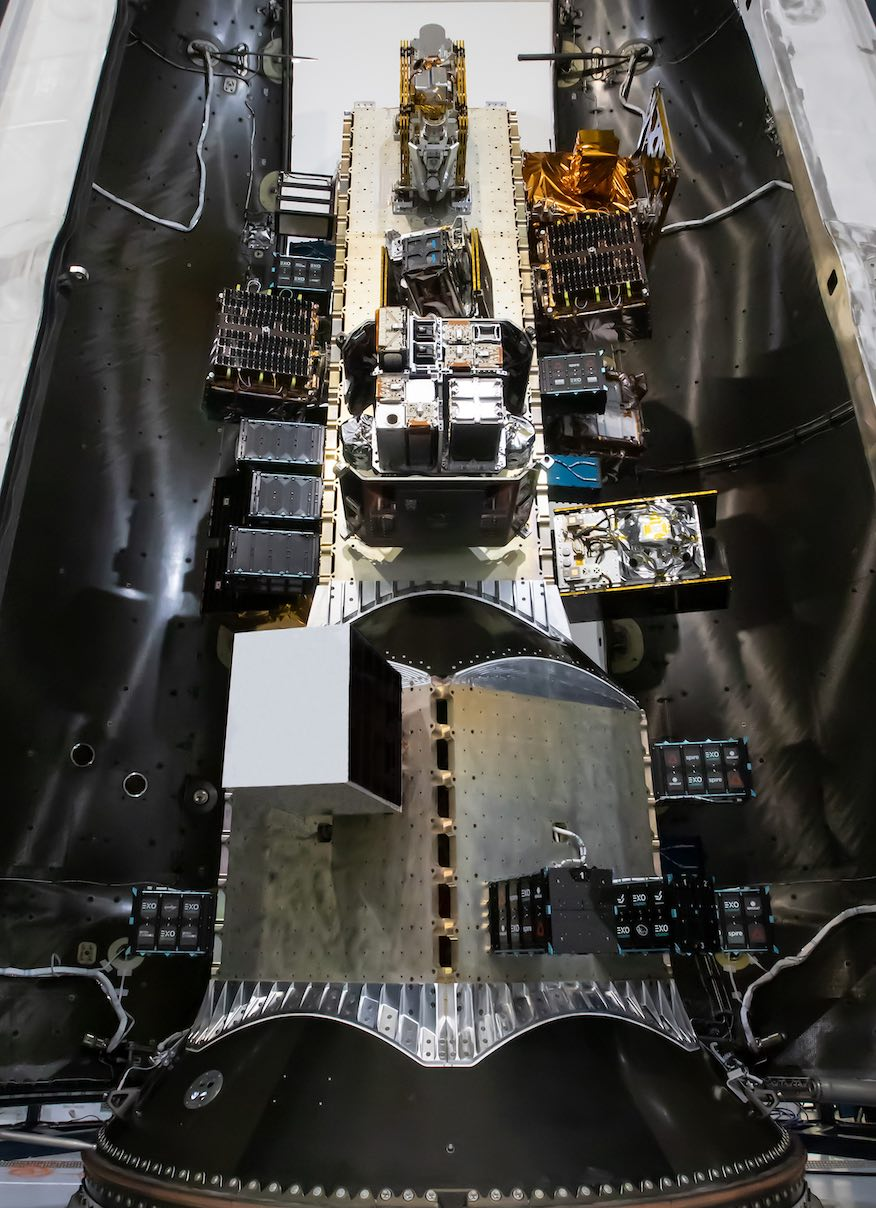
\includegraphics[width=0.8\linewidth]{6.Lanzadores/Transporter-9_small-735101042.jpg}
        \caption{Programa rideshare de SpaceX\\ Fuente: \cite{SFNow_Transporter9_2023}.}
        \label{fig:imagen1}
    \end{minipage}
    \hfill
    \begin{minipage}[t]{0.5\textwidth}
        \centering
        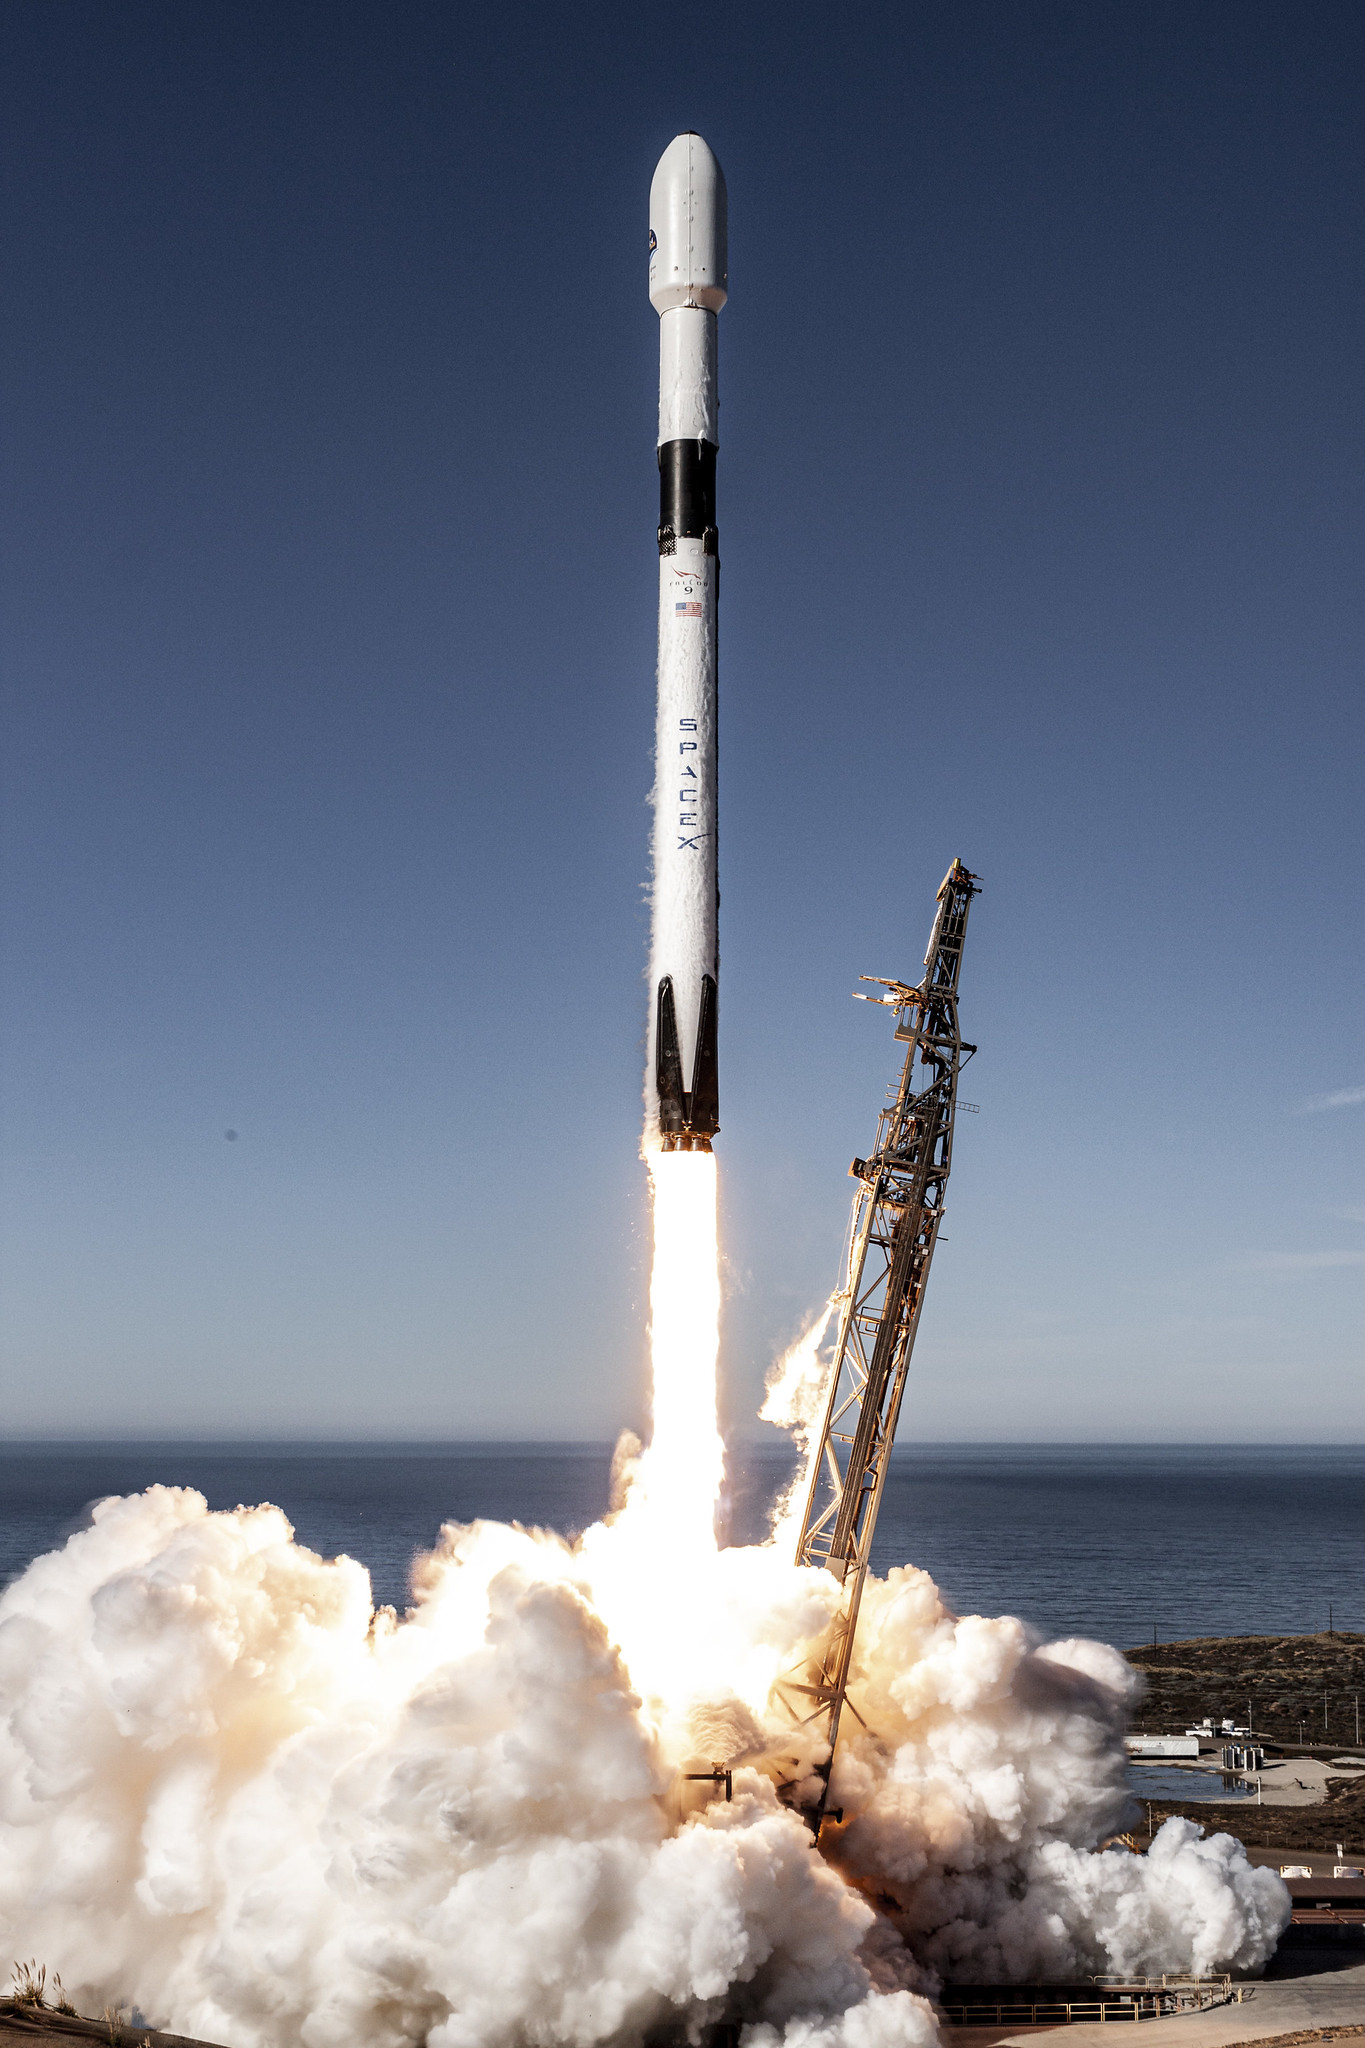
\includegraphics[width=0.8\linewidth]{6.Lanzadores/Copernicus_Sentinel-6_lifts_off_on_a_SpaceX_Falcon_9_rocket-3548914818.jpg}
        \caption{Falcon 9 de SpaceX despegando.\\ Fuente: \cite{wikipedia2024}.}
        \label{fig:imagen2}
    \end{minipage}
\end{figure}

La decisión final recae en el \textbf{Falcon 9} no solo por factores económicos, sino también operativos. Su segunda etapa criogénica ofrece una ventana de reignición de hasta 6 horas, permitiendo ajustes finos de la órbita para optimizar el \textit{swath} de cobertura, así como poner en la orbita deseada ambos satélites. Además, la reutilización de la primera etapa reduce el coste marginal por misión. La alta fiabilidad, así como el programa de \textit{rideshare} y compatibilidad de \textit{dispensers}, permite bajar el coste de lanzamiento en torno a los 26.000 USD, haciendo del lanzador la mejor opción.

La base de lanzamiento de \textbf{Vandenberg SFB} permitirá lanzar dicho vehículo a la órbita requerida, muy utilizada para órbitas polares o heliosíncronas, y que ya está adaptada para el lanzador elegido. Esto nos ayuda a evitar el sobrecoste al existir ya en el lugar la infraestructura, logística, \textit{supply chain}, y personal cualificado para el lanzamiento del Falcon 9.
\newpage

Además, en un entorno geopolítico donde el espacio se ha transformado en un ámbito crucial para la seguridad nacional, optar por lanzadores como el Soyuz-2.1b ruso o el Vega-C europeo podría comprometer el control sobre operaciones sensibles y estratégicas estadounidenses. El Falcon 9, desarrollado y operado por la empresa nacional SpaceX, refuerza la autonomía estratégica de Estados Unidos, consolidando su liderazgo en la industria espacial y disminuyendo la dependencia de actores extranjeros. Esta decisión también promueve el crecimiento de la industria espacial estadounidense, asegurando que los recursos invertidos en la misión favorezcan directamente a la economía nacional y fortalezcan las capacidades tecnológicas internas.

\subsubsection{Azimut de lanzamiento}

Para validar este lanzamiento se puede calcular el azimut de lanzamiento, y comprobar que es viable. Mediante la ecuación:

\begin{equation}
    cos (i) = sin(Az) \cdot \cos(\theta)
\end{equation}

Siendo $i= 97,48 \degree$ la inclinación de interés, $\theta=34,7 \degree$, la latitud a la que se sitúa la base de lanzamiento de Vanderberg SFB, se obtiene un azimut $Az = 198 \degree$. Esto es compatible con los rangos disponibles de la base de lanzamiento \cite{karabeyoglu2018lecture7}.
\begin{figure}[H]
    \centering
    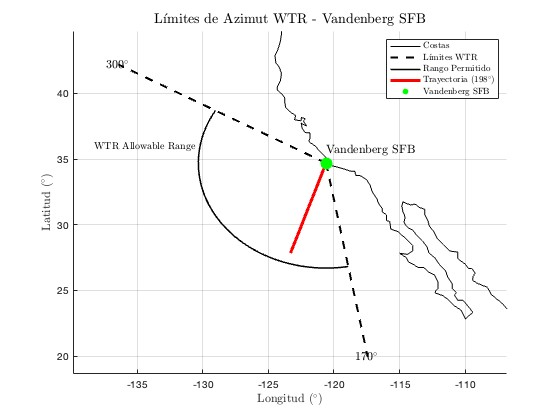
\includegraphics[width=0.7\linewidth]{6.Lanzadores/azimuth.jpg}
    \caption{Azimut de lanzamiento desde Vanderberg SFB. \\Fuente: Elaboración propia.}
    \label{fig:azimut}
\end{figure}

\subsubsection{Despliegue de dos satélites en órbita}

El despliegue de dos satélites en la misma órbita requiere una estrategia de maniobras de fase ejecutada por la etapa superior del lanzador para conseguir el desfase de anomalía. Este procedimiento es habitual en la conformación de constelaciones de satélites y garantiza que ambos compartan idénticos parámetros orbitales, diferenciándose únicamente en su posición relativa sobre la órbita. Se ejecuta en 3 maniobras: 
\begin{enumerate}
    \item Inserción orbital y primer despliegue. El lanzador coloca la etapa superior y los satélites en la órbita objetivo, que en este caso es una SSO circular a 520 km de altitud. Inmediatamente tras alcanzar la órbita, se procede al despliegue del primer satélite, que comienza su operación en la trayectoria planificada.

    \item Maniobra de fase (\textit{Phasing Maneuver}): Tras el primer despliegue, la etapa superior ejecuta una maniobra para modificar temporalmente su órbita. Esta maniobra consiste en ajustar el semieje mayor de la órbita (aumentando el apogeo), lo que genera una diferencia de periodo respecto a la órbita nominal. 

    \item Re-circularización y segundo despliegue: Una vez alcanzada la separación angular de 180°, la etapa superior realiza una nueva maniobra para regresar a la órbita original de 520 km, igualando así todos los elementos orbitales al del primer satélite. Tras estabilizar la órbita, se procede al despliegue del segundo satélite.
\end{enumerate}

A continuación se presenta una simulación en el que, mediante esta maniobra, se consigue el desfase deseado en 37 horas, por medio de una orbita de fase con perigeo en 520 km y apogeo ligeramente más elevado, en 720 km:
\begin{figure}[H]
    \centering
    \begin{minipage}[t]{0.48\textwidth}
        \centering
        \begin{lstlisting}[basicstyle=\tiny\ttfamily]
            >> phaseinjection
            --- Analisis de la Maniobra de Fase ---
            Periodo de la orbita final: 94.88 minutos
            Periodo de la orbita de fase: 96.95 minutos
            Tiempo requerido para un desfase de 180: 36.98 horas
            Numero de orbitas en la trayectoria de fase: 22.89
            -------------------------------------------
        \end{lstlisting}
    \end{minipage}
    \hfill
    \begin{minipage}[t]{0.48\textwidth}
        \centering
        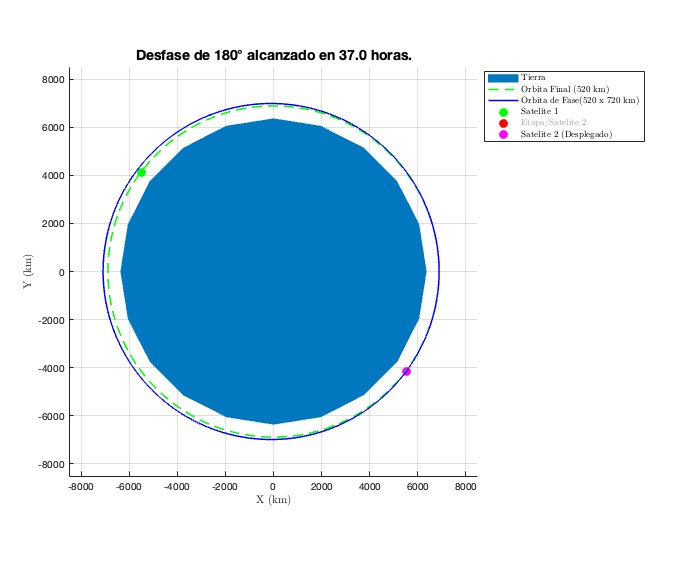
\includegraphics[width=\linewidth]{6.Lanzadores/phasing.jpg}
        \caption{Órbita de fase para el despliegue de los satélites.\\Fuente: Elaboración propia.}
        \label{fig:phasing}
    \end{minipage}
\end{figure}
